%% -------------------------------------
%%
%% Results chapter file.
%%
%% ---------------------
%% Change log:
%% 	2026-03-15 - initial version.
%%
%% ---------------------
%% Authors:
%% 	Santiago Husain Cerruti - hola dot santiago at proton dot me
%%
%% ---------------------
%% Filename: main-body-chapter-results.tex
%% Part of FIUBA-thesis project.
%% Copyright (c) 2026 Santiago Husain Cerruti.
%% Licensed under the MIT License.
%% See LICENSE file for full text.
% -------------------------------------
\chapter{Resultados}

Nullam sed porta risus. Nulla non metus quis quam porta laoreet. Donec egestas nisl purus, a dignissim neque venenatis tempor. Proin facilisis quam eget sem vulputate ultrices. Aliquam sed enim id enim tincidunt sodales eget in enim. Nulla eget finibus libero. Fusce non tristique elit, eget varius erat. Pellentesque malesuada, nulla non rhoncus condimentum, leo nisi sagittis lacus, vel lobortis eros est pretium neque. Nulla nunc justo, convallis sed nibh sit amet, bibendum consectetur lacus.

\section{Sección}\label{section}

Lorem ipsum dolor sit amet, consectetur adipiscing elit. Quisque semper arcu vel enim consectetur, facilisis feugiat dolor bibendum. Donec commodo lacus eget elit dapibus, a venenatis felis consequat. Aliquam consectetur lectus eu dui volutpat scelerisque. Sed laoreet nisi in magna eleifend tempus. Ut ac urna nec nunc tincidunt cursus sit amet eu purus. Sed convallis gravida mi, egestas finibus felis tempus vel. Donec odio sem, laoreet eget maximus elementum, commodo in mi. Pellentesque ut placerat ante. In eu justo eget ligula bibendum molestie eget in nulla. Nam malesuada nisl orci, elementum vulputate nisl pharetra sit amet. Nulla sit amet viverra tortor, a volutpat quam. Nulla quis mauris a justo consequat gravida. Donec posuere lorem id consectetur egestas.


\begin{lstlisting}[language=C++, style=StyleC,caption={Snippet: \texttt{MathsDefinitions.hpp}.},captionpos=b,label={MathsDefinitions}]
	#ifndef ORBIT_GENERATOR_MATHSDEFINITIONS_HPP
	#define ORBIT_GENERATOR_MATHSDEFINITIONS_HPP
	
	#include <eigen3/Eigen/Dense>
	
	using Vector3D = Eigen::Matrix<double, 3, 1>;
	using Vector3LD = Eigen::Matrix<double, 3, 1>;
	using Vector6D = Eigen::Matrix<double, 6, 1>;
	using Vector6LD = Eigen::Matrix<double, 6, 1>;
	using Matrix3D = Eigen::Matrix<double, 3, 3>;
	using Matrix3LD = Eigen::Matrix<double, 3, 3>;
	using MatrixXLD = Eigen::Matrix<double, Eigen::Dynamic, Eigen::Dynamic>;
	using MatrixXD = Eigen::Matrix<double, Eigen::Dynamic, Eigen::Dynamic>;
	using VectorXD = Eigen::Matrix<double, Eigen::Dynamic, 1>;
	using RotationMatrixLD = Eigen::Matrix<double, 3, 3>;
	
	#endif  // ORBIT_GENERATOR_MATHSDEFINITIONS_HPP
\end{lstlisting}

Nullam sed porta risus. Nulla non metus quis quam porta laoreet. Donec egestas nisl purus, a dignissim neque venenatis tempor. Proin facilisis quam eget sem vulputate ultrices. Aliquam sed enim id enim tincidunt sodales eget in enim. Nulla eget finibus libero. Fusce non tristique elit, eget varius erat. Pellentesque malesuada, nulla non rhoncus condimentum, leo nisi sagittis lacus, vel lobortis eros est pretium neque. Nulla nunc justo, convallis sed nibh sit amet, bibendum consectetur lacus.

\subsection{Subsección}

Nullam sed porta risus. Nulla non metus quis quam porta laoreet. Donec egestas nisl purus, a dignissim neque venenatis tempor. Proin facilisis quam eget sem vulputate ultrices. Aliquam sed enim id enim tincidunt sodales eget in enim. Nulla eget finibus libero. Fusce non tristique elit, eget varius erat. Pellentesque malesuada, nulla non rhoncus condimentum, leo nisi sagittis lacus, vel lobortis eros est pretium neque. Nulla nunc justo, convallis sed nibh sit amet, bibendum consectetur lacus.


\begin{figure}[t]
	\centering
	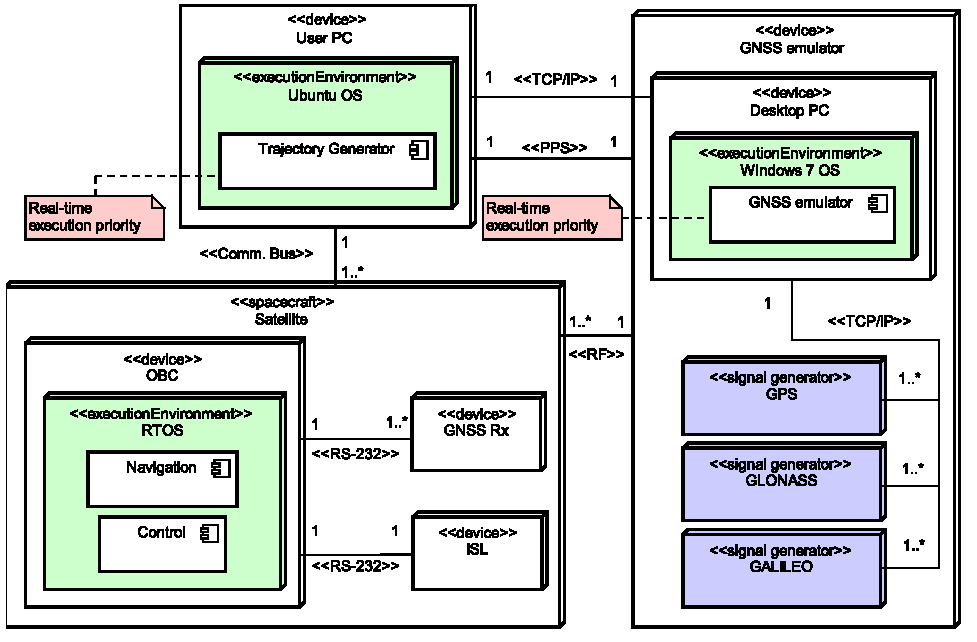
\includegraphics[scale=0.7]{media/main-body-chapter-results/fig-testbed-deployment-diagram-HIL.pdf}
	\caption{Testbed deployment.}\label{figure}
\end{figure}


\begin{lstlisting}[language=C++, style=StyleC, caption={Snippet}]
	typedef boost::interprocess::deque<Command, allocator_t> deque_t;
	typedef boost::interprocess::interprocess_mutex mutex_t;
	typedef boost::interprocess::scoped_lock<mutex_t> scoped_lock_t;
	typedef boost::interprocess::managed_shared_memory managed_shared_memory_t;
\end{lstlisting}

Nullam sed porta risus. Nulla non metus quis quam porta laoreet. Donec egestas nisl purus, a dignissim neque venenatis tempor. Proin facilisis quam eget sem vulputate ultrices. Aliquam sed enim id enim tincidunt sodales eget in enim. Nulla eget finibus libero. Fusce non tristique elit, eget varius erat. Pellentesque malesuada, nulla non rhoncus condimentum, leo nisi sagittis lacus, vel lobortis eros est pretium neque. Nulla nunc justo, convallis sed nibh sit amet, bibendum consectetur lacus.

\begin{lstlisting}[language=C++, style=StyleC,caption={Snippet: Definiciones de \texttt{TimeScale} y \texttt{TimeFormat} y comandos de control.},captionpos=b,label={defs_TimeScale_TimeFormat}]
	typedef enum TimeScale
	{
		UT1,
		UTC,
		TT,
		Uniform,
		InvalidTimeScale
	} TimeScale;
	
	typedef enum TimeFormat
	{
		Gregorian,
		MJD,
		ElapsedTime,
		InvalidTimeFormat
	} TimeFormat;
	
	try
	{
		boost::optional<ControlCommand> _command;
		_command = _queue->try_pop();
		if (_command)
		_currentCommand = *_command;
	}
	catch (const std::exception& e)
	{
		std::cerr << "ERROR: ContinuousThruster::getActuatorAcceleration(): " << e.what();
	}	
\end{lstlisting}

Nullam sed porta risus. Nulla non metus quis quam porta laoreet. Donec egestas nisl purus, a dignissim neque venenatis tempor. Proin facilisis quam eget sem vulputate ultrices. Aliquam sed enim id enim tincidunt sodales eget in enim. Nulla eget finibus libero. Fusce non tristique elit, eget varius erat. Pellentesque malesuada, nulla non rhoncus condimentum, leo nisi sagittis lacus, vel lobortis eros est pretium neque. Nulla nunc justo, convallis sed nibh sit amet, bibendum consectetur lacus.

\begin{lstlisting}[style=StyleC, caption={Snippet: Mi código en C++}]
	int main() {
		return 0; // Hola mundo
	}
\end{lstlisting}

Nullam sed porta risus. Nulla non metus quis quam porta laoreet. Donec egestas nisl purus, a dignissim neque venenatis tempor. Proin facilisis quam eget sem vulputate ultrices. Aliquam sed enim id enim tincidunt sodales eget in enim. Nulla eget finibus libero. Fusce non tristique elit, eget varius erat. Pellentesque malesuada, nulla non rhoncus condimentum, leo nisi sagittis lacus, vel lobortis eros est pretium neque. Nulla nunc justo, convallis sed nibh sit amet, bibendum consectetur lacus.

\begin{lstlisting}[language=yaml, caption={Snippet: Configuración YAML}]
	host: localhost
	port: 8080
\end{lstlisting}

Nullam sed porta risus. Nulla non metus quis quam porta laoreet. Donec egestas nisl purus, a dignissim neque venenatis tempor. Proin facilisis quam eget sem vulputate ultrices. Aliquam sed enim id enim tincidunt sodales eget in enim. Nulla eget finibus libero. Fusce non tristique elit, eget varius erat. Pellentesque malesuada, nulla non rhoncus condimentum, leo nisi sagittis lacus, vel lobortis eros est pretium neque. Nulla nunc justo, convallis sed nibh sit amet, bibendum consectetur lacus.

\begin{lstlisting}[style=terminal, caption={Vista desde una terminal Linux.}]
	$ g++ -Wall -pedantic main.cpp -o programa
	$ ./programa
	Hola Mundo!
\end{lstlisting}


\begin{algorithm}[t]
	\caption{Pseudocódigo del algoritmo AROM.}\label{alg_AROM}
	\begin{algorithmic}[1]
		\Require Posiciones y velocidades actuales de los satélites líder y seguidor.
		\Ensure  Comando de actuación.
		\Statex
		\Procedure{AROM}{}
		\Statex
		\State A partir de las posiciones y velocidades actuales del líder y seguidor, calcular sus elementos orbitales osculates $\xi_c$ y $\xi_d$, respectivamente, con $\xi = \left[a,\lambda_U,h_U,l_U,i,\Omega\right]^t$.
		\Statex
		\State Obtener los MOE $\bar{\xi}_c$ y $\bar{\xi}_d$ utilizando el algoritmo de Spiridonova con las perturbaciones.
		\Statex
		\State Calcular los MOE de la maniobra deseada actual como $\bar{\xi}_m(t) = \bar{\xi}_c + \delta_m^c\xi(t)$.
		\Statex
		\State Calcular el error MOE del seguidor respecto de la maniobra $\delta_d^m \bar{\xi} = \bar{\xi}_d - \bar{\xi}_m$, y del seguidor respecto del líder $\delta_d^c \bar{\xi} = \bar{\xi}_d - \bar{\xi}_c$.
		\Statex
		\State Etc..
		\Statex
		\EndProcedure
	\end{algorithmic}
\end{algorithm}
